%! TEX root = ../curbe.tex

\chapter{Curbe eliptice}

\section{Ecuații Weierstrass}
\todo[inline,noline,backgroundcolor=green!40]{chiar e necesar? -- păstrează minimum pt.\ Schoof!}

Vom studia în special curbe eliptice, care sînt curbe de gen 1,
cu un punct-bază specificat. Vom vedea că orice astfel de curbă poate
fi gîndită ca locul geometric în $ \PP^2 $ al unei ecuații cubice cu un punct,
punctul bază, pe linia de la infinit. Apoi, după o schimbare de coordonate,
orice curbă eliptică se poate prezenta sub forma:
\[
      Y^2Z + a_1 XYZ + a_3 YZ^2 = X^3 + a_2X^2Z + a_4XZ^2 + a_6Z^3.
\]
În acest caz, punctul bază este $ O = [0, 1, 0] $, iar $ a_i \in \overline{K} $.

Studiem acum curbele eliptice care sînt date cu formule explicite,
numite \emph{ecuații Weierstrass}.

Pentru simplificarea notației, vom lucra cu coordonatele neomogene,
$ x = X/Z $ și $ y = Y/Z $ și atunci, putem scrie curba:
\[
      E : y^2 + a_1 xy + a_3 y = x^3 + a_2 x^2 + a_4 x + a_6,
\]
ținînd cont și de un punct $ O = [0, 1, 0] $ la infinit. Ca în cazul
oricărei varietăți, dacă $ a_i \in K $, spunem că avem o curbă $ E $
\emph{definită peste $ K $}.

Presupunem că lucrăm cu $ \dr{char}(\overline{K}) \neq 2 $ și atunci
putem simplifica ecuația, cu substituția:
\[
    y \mapsto \dfrac{1}{2} \left( y - a_1x - a_3 \right),
\]
care conduce la ecuația:
\[
      E : y^2 = 4x^3 + b_2 x^2 + 2b_4 x + b_6,
\]
cu notațiile:
\[
      b_2 = a_1^2 + 4a_4, \quad b_4 = 2a_4 + a_1a_3, \quad b_6 = a_3^2 + 4a_6.
\]
Mai definim și:
\begin{align*}
    b_8 &= a_1^2 a_6 + 4a_2a_6 - a_1a_3a_4 + a_2a_3^2 - a_4^2 \\
    c_4 &= b_2^2 - 24b_4 \\
    c_6 &= -b_2^3 + 36b_2b_4 - 216b_6 \\
    \Delta &= -b_2^2b_8 - 8b_4^3 - 27b_6^2 + 9b_2b_4b_6 \\
    j &= c_4^3 / \Delta \\
    \omega &= \dfrac{dx}{2y + a_1x + a_3} = \dfrac{dy}{3x^2 + 2a_2x + a_4 - a_1y}.
\end{align*}

Relațiile simple între aceste cantități sînt:
\[
    4b_8 = b_2b_6 - b_4^2, \quad \text{și} \quad 1728\Delta = c_4^3 - c_6^2.
\]

Mai departe, dacă $ \dr{char}\overline{K} \neq 2, 3 $, putem face substituția:
\[
    (x, y) \mapsto \left( \dfrac{x - 3b_2}{36}, \dfrac{y}{108} \right),
\]
care elimină termenul cu $ x^2 $ și ajungem la:
\[
      E : y^2 = x^3 - 27c_4x - 54c_6.
\]

\begin{definition}\label{def:invarianti-weierstrass}
    \index{invariant Weierstrass!discriminant}
    \index{invariant Weierstrass!j}
    \index{invariant Weierstrass!diferențial}
    Cantitatea $ \Delta $ se numește \emph{discriminantul} ecuației Weierstrass,
    cantitatea $ j $ se cheamă $ j $-invariantul curbei eliptice, iar
    $ \omega $ este \emph{invariantul diferențial} asociat ecuației.
\end{definition}

Considerăm acum o situație generală. Fie $ P = (x_0, y_0) $ un punct arbitrar care
satisface o ecuație de tip Weierstrass:
\[
    f(x, y) = y^2 + a_1 xy + a_3 y - x^3 - a_2x^2 - a_4 x - a_6 = 0
\]
și mai presupunem că $ P $ este o singularitate pentru curba $ f(x, y) = 0 $, deci
\[
    \dfrac{\partial f}{\partial x}(P) = \dfrac{\partial f}{\partial y}(P) = 0.
\]
Rezultă că există coeficienți $ \alpha, \beta \in \overline{K} $ astfel încît
dezvoltarea Taylor a polinomului $ f(x, y) $ în jurul lui $ P $ se poate scrie:
\[
    f(x, y) - f(x_0, y_0) = ((y - y_0) - \alpha(x - x_0))((y - y_0) - \beta(x - x_0)) - %
    (x - x_0)^3.
\]

\begin{definition}\label{def:nod}
    Folosind notațiile de mai sus, singularitatea $ P $ se numește \emph{nod} dacă
    $ \alpha \neq \beta $, iar în acest caz, curbele:
    \[
        y - y_0 = \alpha(x - x_0) \quad \text{și} \quad y - y_0 = \beta(x - x_0)
    \]
    se numesc \emph{tangentele în $ P $}. Reciproc, dacă $ \alpha = \beta $,
    spunem că $ P $ este \emph{vîrf} (eng.\ \textit{cusp}), caz în care
    tangenta la $ P $ este dată de:
    \[
        y - y_0 = \alpha(x - x_0).
    \]
\end{definition}

%%%%%%%%%%%%%%%%%%%%%%%%%%%%%%%%%%%%%%%%%%%%%%%%%%%%%%%%%%%%%%%%%%%%%%
\section{Structura de grup}

Fie $ E $ o curbă eliptică dată de o ecuație Weierstrass. Rezultă că
$ E \seq \PP^2 $ conține puncte $ P = (x, y) $ care satisfac ecuația
Weierstrass, împreună cu punctul $ O = [0, 1, 0] $ de la infinit.

Fie $ L \seq \PP^2 $ o dreaptă. Atunci, deoarece ecuația are gradul 3,
dreapta $ L $ intersectează $ E $ în exact 3 puncte, pe care le notăm
$ P, Q, R $.

\begin{definition}\label{def:adunare-eliptic}
    Fie $P, Q \in E $ și fie $ L $ dreapta prin $ P $ și $ Q $ (dacă $ P = Q $,
    atunci $ L $ este tangenta în $ P $). Fie $ R $ un al treilea punct
    de intersecție a lui $ L $ cu $ E $.

    Fie $ L' $ dreapta prin $ R $ și $ O $. Atunci $ L' $ intersectează
    $ E $ în $ R, O $ și un al treilea punct. Acest al treilea punct se notează
    $ P \oplus Q $.
\end{definition}

Operația este ilustrată în figura \ref{fig:adunare-el}.
\begin{figure}[!htbp]
    \centering
    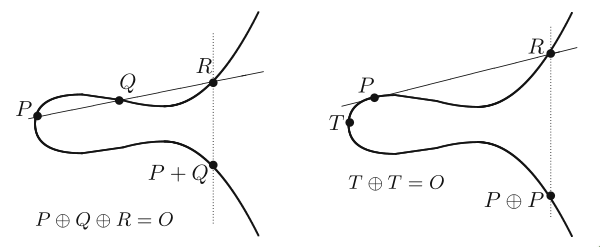
\includegraphics[scale=0.5]{figs/adunare-el.png}
    \caption{\textit{Adunarea punctelor pe o curbă eliptică, \cite{sil09}, p.\ 51}}
    \label{fig:adunare-el}
\end{figure}

Cu acestea, se obține că $ (E, \oplus) $ formează un grup abelian, cu elementul
neutru $ O = [0, 1, 0] $. Pentru simplitate, în continuare vom nota operațiile
cu notațiile obișnuite, $ \oplus \mapsto +, \ominus \mapsto - $.

\begin{example}\label{exm:eliptic-grup}
    Fie curba eliptică $ E/\QQ $:
    \[
          E : y^2 = x^3 + 17.
    \]
    Calcule simple găsesc cîteva puncte cu coordonate întregi:
    \[
        P_1 = (-2, 3), P_2 = (-1, 4), P_3 = (2, 5), P_4 = (4, 9), P_5 = (8, 23).
    \]
    Folosind operația de grup, se pot verifica relațiile:
    \[
          P_5 = -2 \cdot P_1, \quad P_4 = P_1 - P_3.
    \]
    Se poate arăta că orice punct rațional $ P \in E(\QQ) $ poate fi scris sub forma:
    \[
          P = mP_1 + nP_3, \quad m, n \in \ZZ,
    \]
    ceea ce ne arată că $ E(\QQ) \simeq \ZZ \times \ZZ $.
\end{example}

%%%%%%%%%%%%%%%%%%%%%%%%%%%%%%%%%%%%%%%%%%%%%%%%%%%%%%%%%%%%%%%%%%%%%
\section{Curbe eliptice}

Fie $ E $ o curbă netedă de gen 1.

\begin{definition}\label{def:curba-el}
    O \emph{curbă eliptică} este o pereche $ (E, O) $, alcătuită dintr-o
    curbă nesingulară $ E $ de gen 1 și un punct $ O \in E $.

    Curba se numește \emph{definită peste corpul $ K $}, notat $ E/K $,
    dacă $ E $ este o curbă definită peste $ K $, iar $ O \in E(K) $.
\end{definition}

Relevanța ecuației Weierstrass reiese din:
\begin{proposition}\label{prop:weierstrass-eliptic}
    Fie $ E $ o curbă eliptică definită peste $ K $.
    \begin{enumerate}[(a)]
        \item Există funcțiile $ x, y \in K(E) $ astfel încît aplicația:
            \[
                \phi : E \to \PP^2, \quad \phi = [x, y, 1]
            \]
           dă un izomorfism între $ E/K $ și o curbă dată de o ecuație Weierstrass:
           \[
               C : Y^2 + a_1 XY + a_3 Y = X^3 + a_2 X^2 + a_4 X + a_6,
           \]
           cu coeficienții $ a_1, \dots, a_6 \in K $ și $ \phi(O) = [0, 1, 0] $.

           Funcțiile $ x, y $ se numesc \emph{coordonatele Weierstrass} ale
           curbei eliptice $ E $.
       \item Orice două ecuații Weierstrass pentru curba fixată $ E $ sînt
           legate printr-o schimbare de variabile de forma:
           \[
                 X = u^2 X' + r, \quad Y = u^3 Y' + su^2 X' + t,
           \]
           pentru $ u \in K^\times, r, s, t \in K $.
       \item Reciproc, orice curbă cubică netedă $ C $ dată de o ecuație
           Weierstrass ca în (a) este o curbă eliptică definită peste $ K $,
           cu punctul bază $ O = [0, 1, 0] $.
    \end{enumerate}
\end{proposition}

\begin{corollary}\label{cor:weier-eliptic}
    Fie $ E/K $ o curbă eliptică cu coordonatele Weierstrass $ x, y $ ca în
    teoremă. Atunci:
    \[
        K(E) = K(x, y) \quad \text{și} \quad [K(E) : K(x)] = 2.
    \]
\end{corollary}

\todo[inline,noline,backgroundcolor=green!40]{cam puțin...}



%%% Local Variables:
%%% mode: latex
%%% TeX-master: "../curbe"
%%% End:
